% status: 80
% chapter: TBD

\title{Automated Spark Cluster Deployment on EC2}


\author{Sandeep Khandelwal}
\affiliation{%
  \institution{Indiana University}
  \city{Bloomington} 
  \state{IN} 
  \postcode{47408}
  \country{USA}}
\email{skhande@iu.edu}



% The default list of authors is too long for headers}
\renewcommand{\shortauthors}{Sandeep}


\begin{abstract}

This project is about developing a module for automated deployment of
Apache Spark cluster on AWS (Amazon Web Services) EC2 (Elastic Compute
Cloud) instances on a single click and perform various data processing
related tasks on Apache Spark Cluster. This project provide option to
terminate the Apache Spark cluster once data processing task is
completed. This project also does the benchmarking of deployment, data
processing and termination of the instances.

\end{abstract}

\keywords{AWS, EC2, Apache Spark, Apache Hadoop, Ansible}


\maketitle

\section{Introduction}

This module does infrastructure related tasks of provisioning of
AWS~\cite{hid-sp18-511-www-aws} EC2~\cite{hid-sp18-511-www-ec2}
instances, setting up the public/private key pair for secure
connection with EC2~\cite{hid-sp18-511-www-ec2} instance and configure
inbound/outbound traffic rules on provisioned machines to allow
connectivity on various ports. This module also perform Apache
Spark~\cite{hid-sp18-511-www-spark} installation on the provisioned
EC2~\cite{hid-sp18-511-www-ec2} instances using master/worker model
and perform all required configuration. One of the machine will work
as a master node and other machines will work as worker node. User can
do various data processing related tasks once Apache
Spark~\cite{hid-sp18-511-www-spark} cluster is setup. Apache
Spark~\cite{hid-sp18-511-www-spark} cluster can be terminated once
data processing related task complete.

The module expose command line options for Apache
Spark~\cite{hid-sp18-511-www-spark} cluster deployment and termination
of machines. User can connect to Apache
Spark~\cite{hid-sp18-511-www-spark} cluster and perform various data
related tasks. Benchmarking is done for measuring the deployment, data
processing and termination of the instances.

Ansible~\cite{hid-sp18-511-www-ansible} automation tool is be used in
this project to provision EC2~\cite{hid-sp18-511-www-ec2} instances,
deploy Apache Spark~\cite{hid-sp18-511-www-spark} cluster on
EC2~\cite{hid-sp18-511-www-ec2} instance and perform various data
processing related tasks on Apache Spark~\cite{hid-sp18-511-www-spark}
cluster.

\section{Technologies Used}
This section describes the technology used in the project.

\begin{itemize}
	\item[$\bullet$] AWS 
	\item[$\bullet$] Apache Spark 
	\item[$\bullet$] Ansible
\end{itemize}

\section{AWS}

AWS~\cite{hid-sp18-511-www-aws} is a secure cloud service provider
that provide various on-demand services.
AWS~\cite{hid-sp18-511-www-aws} provides services in Compute, Storage,
Database, Migration, Networking and Content Delivery, Developer Tools
and many more. These services are easy to setup and can be configured
in few minutes. All the services are on demand service and
AWS~\cite{hid-sp18-511-www-aws} charge only for the duration service
is being used. This is very effective and suitable for both small and
large customers.

The following configuration is used in this project:

\begin{itemize}
	\item \verb|project_name: ec2_spark|
	\item \verb|region: us-west-2|
	\item \verb|env: stg|
\end{itemize}


\subsection{EC2}

EC2~\cite{hid-sp18-511-www-ec2} is AWS secure and re sizable compute
service. EC2~\cite{hid-sp18-511-www-ec2} instances can be created on
demand with different configuration of memory, CPU power and hard
disk. EC2~\cite{hid-sp18-511-www-ec2} instances can be added and
terminated at run time based on the load of application. Adding or
terminating EC2~\cite{hid-sp18-511-www-ec2} instances is very easy and
can be done in few minutes.

Two EC2~\cite{hid-sp18-511-www-ec2} instances are created in this
project with following configuration. One of the instance is used for
master node and another one for worker node.

Table~\ref{t:ec2-configuration} provides the
EC2~\cite{hid-sp18-511-www-ec2} configuration details.

\begin{table}[]
	\centering \caption{Configuration}\label{t:ec2-configuration}
        \begin{tabular}{lllll} \textbf{Node}
	& \textbf{AMI} & \textbf{CPUs} & \textbf{RAM}
	& \textbf{Disk}\\ Apache Spark Master & ami-4e79ed361 & 1 & 2
	GB & 8GB\\ Apache Spark Worker & ami-4e79ed361 & 1 & 2 GB &
	8GB\\ \end{tabular}
\end{table}

\subsection{Security Group}

Security Group restrict the inbound and outbound traffic for
EC2~\cite{hid-sp18-511-www-ec2} instance.  We can define the allowed
incoming and outgoing traffic using Security Group and assign it to
the instance.  Security Group works as firewall and allow only
permitted traffic on EC2~\cite{hid-sp18-511-www-ec2} instance.

\verb|ec2_spark_stg_security_group| Security group is created with the
following inbound and outbound ports open in this project and assigned
to the EC2~\cite{hid-sp18-511-www-ec2} instances created

\begin{itemize}
	\item \verb|Inbound: 80, 8080, 22, 7178, 8181, 7077, 443|
	\item \verb|Outbound: all|
	
\end{itemize}

\subsection{Key Pair}

Key Pair is used to connect EC2~\cite{hid-sp18-511-www-ec2}
instance. We need to create Key Pair and provide the private key to
connect the EC2~\cite{hid-sp18-511-www-ec2} instance.

\verb|ec2_spark_stg_key| Key pair is created in this project.
The private key with the name \verb|ec2_spark_stg_key-private.pem| is
created and saved on the user machine and used for making the ssh
connection to EC2~\cite{hid-sp18-511-www-ec2} instances.

\section{Apache Spark}

Apache Spark~\cite{hid-sp18-511-www-spark} is analytics engine for
large scale data processing. Apache
Spark~\cite{hid-sp18-511-www-spark} has high performance engine, very
easy to use and provide option to plug-in third party components.

The following configuration is used in this project for Apache Spark

\begin{itemize}
	\item \verb|spark_version: 2.3.0|
	\item \verb|spark_hadoop_version: 2.7|
	\item \verb|spark_temp_dir: /tmp|
	\item \verb|spark_working_dir: /var/lib/spark|
	\item \verb|spark_install_dir: /opt/spark|
	\item \verb|spark_mirror: http://apache.claz.org/|
	\verb|spark/spark-2.3.0/|
	\item \verb|spark_master_memory_mb: 1024|
	\item \verb|spark_master_work_port: 7077|
	\item \verb|spark_master_ui_port: 8080|
	\item \verb|spark_worker_memory_mb: 1024|
	\item \verb|spark_worker_work_port: 7178|
	\item \verb|spark_worker_ui_port: 8181|
\end{itemize}

\section{Ansible}

Ansible~\cite{hid-sp18-511-www-ansible} is open source software for
the infrastructure automation, configuration management and
application deployment. Automation tasks are defined in Ansible
Playbook using YAML language. For communication to hosts,
Ansible~\cite{hid-sp18-511-www-ansible} uses OpenSSH\@.

For this project Ansible~\cite{hid-sp18-511-www-ansible} is used to
create and setup EC2~\cite{hid-sp18-511-www-ec2} instances, deploy
Apache Spark~\cite{hid-sp18-511-www-spark} cluster on
EC2~\cite{hid-sp18-511-www-ec2} instance and perform various data
processing related tasks on Apache Spark~\cite{hid-sp18-511-www-spark}
Cluster and terminate Apache Spark~\cite{hid-sp18-511-www-spark}
cluster.

\section{Deployment}

\subsection{Setup}

\paragraph{Ansible}
Download and install Ansible~\cite{hid-sp18-511-www-ansible} on the
machine where deployment script will be executed.

Ansible~\cite{hid-sp18-511-www-ansible} can be downloaded from
\url{https://www.ansible.com/resources/get-started}

Download and install Ansible from the above URL and validate the
installation by typing:

\begin{verbatim}
$ ansible-playbook --version
\end{verbatim}

You should see the following output. Version number and directories
could be different in your case.

\begin{verbatim}
ansible-playbook 2.5.0 version = 2.7.13
(default, Jan 24 2018, 21:48:31) [GCC 5.4.0 20160609]
\end{verbatim}

\paragraph{AWS key}

Create AWS account if not exist already and get the
AWS~\cite{hid-sp18-511-www-aws} ID and secret key. These keys will be
used in authentication with AWS~\cite{hid-sp18-511-www-aws}.

Provide the values for
\verb|AWS_ACCESS_KEY_ID| and \verb|AWS_SECRET_ACCESS_KEY|.

Enter the information on command line:

\begin{verbatim}
export AWS_ACCESS_KEY_ID='<AWS_ACCESS_KEY_ID value>' 
export
AWS_SECRET_ACCESS_KEY='<AWS_SECRET_ACCESS_KEY value>'
\end{verbatim}

Validate the variable by typing the following command:
\begin{verbatim}
echo AWS_ACCESS_KEY_ID
echo AWS_SECRET_ACCESS_KEY
\end{verbatim}

You should see the values as output which were previously set by
export command.

\paragraph{Git repository}

Setup the git repository:

\begin{verbatim}
export HID=hid-sp18-511 
mkdir -p ~/github/cloudmesh-community
cd ~/github/cloudmesh-community 
git clone
https://github.com/cloudmesh-community/$HID.git
/project-code
\end{verbatim}

Validate code has been cloned into the directory.

\paragraph{Configuration options}

There are various configuration option that can be updated based on
the requirement.

AWS related configuration options:

\begin{verbatim}
cd ~/github/cloudmesh-community/$HID.git/project-code/
group_vars/all
\end{verbatim}

Open main.yml file and update the following information as per the
requirement:

\begin{verbatim}
project_name: <specify the project name>
region: <specify AWS region>
env: <deployment environment>
\end{verbatim}

EC2 related configuration options:

\begin{verbatim}
cd ~/github/cloudmesh-community/$HID.git/project-code/
roles/provisionec2/defaults
\end{verbatim}

Open main.yml file and update the following information as per the
requirement

\begin{verbatim}
ami_image: <EC2 AMI image type>
instance_type: <Instance type>
\end{verbatim}

Apache Spark~\cite{hid-sp18-511-www-spark} related configuration options:

\begin{verbatim}
cd ~/github/cloudmesh-community/$HID.git/project-code/
roles/sparkmaster/defaults
\end{verbatim}

Open main.yml file and update the following information as per the
requirement

\begin{verbatim}
spark_version: <Spark master version>
spark_hadoop_version: <Hadoop version>
spark_temp_dir: <Spark master temprary directory>
spark_working_dir: <Spark master working directory>
spark_install_dir: <Spark master installation directory>
spark_mirror: <Spark master mirror URL>
spark_master_memory_mb: <Spark master memory>
spark_master_work_port: <Spark master work port>
spark_master_ui_port: <Spark master UI port>
\end{verbatim}

\begin{verbatim}
cd ~/github/cloudmesh-community/$HID.git/project-code/
roles/sparkworker/defaults
\end{verbatim}

Open main.yml file and update the following information as per the
requirement

\begin{verbatim}
spark_version: <Spark worker version>
spark_hadoop_version: <Hadoop version>
spark_temp_dir: <Spark worker temprary directory>
spark_working_dir: <Spark worker working directory>
spark_install_dir: <Spark master installation directory>
spark_mirror: <Spark worker mirror URL>
spark_master_work_port: <Spark master work port>
spark_master_ui_port: <Spark worker UI port>
spark_worker_work_port: <Spark worker work port>
spark_worker_ui_port: <Spark worker UI port>
\end{verbatim}

\subsection{Deploy Apache Spark Cluster}

Execute the following command on the command line to deploy Apache
Spark Cluster~\cite{hid-sp18-511-www-spark}.

\begin{verbatim}
cd ~/github/cloudmesh-community/$HID.git/project-code/
ansible-playbook site.yml --tags ''provision''
\end{verbatim}

This command will perform following tasks:

\begin{itemize}
	\item Create Security Group in AWS
	\item Create Key Pair in AWS
	\item Provision EC2 instance for Spark master
	\item Provision EC2 instance for Spark worker
	\item Create Spark user and group on Spark master
	\item Setup Spark specific directories on Spark master
	\item Download and unarchive Spark on Spark master
	\item Download and install Java on Spark master
	\item Setup Spark configuration files on Spark master
	\item Start Spark master service on Spark master
	\item Create Spark user and group on Spark worker
	\item Setup Spark specific directories on Spark worker
	\item Download and unarchive Spark  on Spark worker
	\item Download and install Java  on Spark worker
	\item Setup Spark configuration files on Spark worker
	\item Spark worker service and add to Spark master	
\end{itemize}

\textbf{Security Group:}

Figure~\ref{f:security-group} shows security group created in the deployment.

\begin{figure}[!ht]
	\centering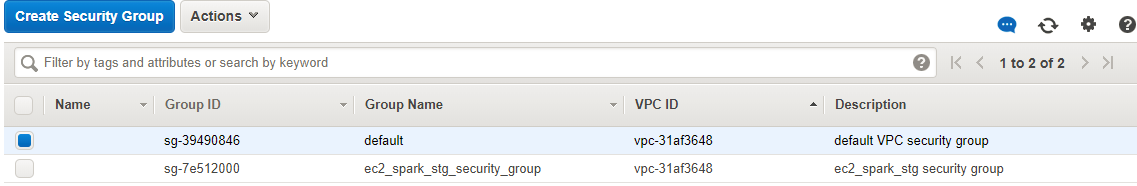
\includegraphics[width=\columnwidth]{images/securitygroup.png}
	\caption{Security group}\label{f:security-group}
\end{figure}

\textbf{Key Pair:}

Figure~\ref{f:key-pair} shows Key pair created in the deployment.

\begin{figure}[!ht]
	\centering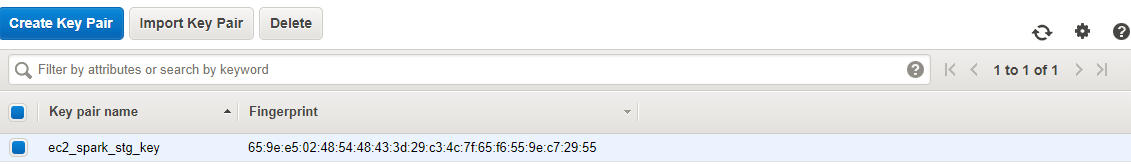
\includegraphics[width=\columnwidth]{images/keypair.png}
	\caption{Key pair}\label{f:key-pair}
\end{figure}

\textbf{EC2~\cite{hid-sp18-511-www-ec2} instances:}

Figure~\ref{f:ec2-instance} shows EC2 instances created in the deployment.

\begin{figure}[!ht]
	\centering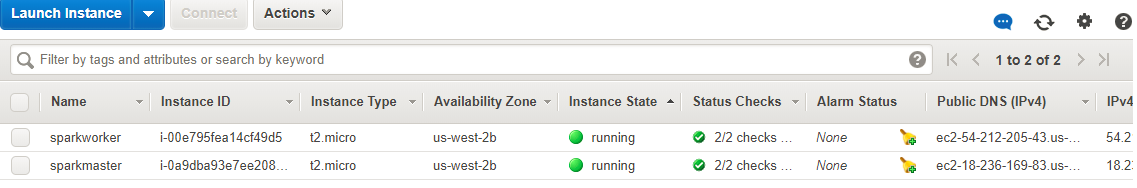
\includegraphics[width=\columnwidth]{images/ec2instances.png}
	\caption{EC2 instance}\label{f:ec2-instance}
\end{figure}


\begin{verbatim}
cd ~/github/cloudmesh-community/$HID.git/project-code/inventory
\end{verbatim}

Open hosts file and find out the IP address in [sparkmaster] and
[sparkworker] section.

Connect to the Spark worker node using ssh:

\begin{verbatim}
ssh -i ec2_spark_stg_key-private.pem ubuntu@<Spark worker IP adddress>
\end{verbatim}

Once you connect to the Spark worker, execute the command:

\begin{verbatim}
sudo start-slave.sh spark://18.236.169.83:7077
\end{verbatim}

Validate Spark Apache cluster up and running by typing the below url
in browser

\begin{verbatim}
http://18.236.169.83:8080
\end{verbatim}

Figure~\ref{f:spark-cluster-url} shows Apache
Spark~\cite{hid-sp18-511-www-spark} cluster URL\@.

\begin{figure}[!ht]
\centering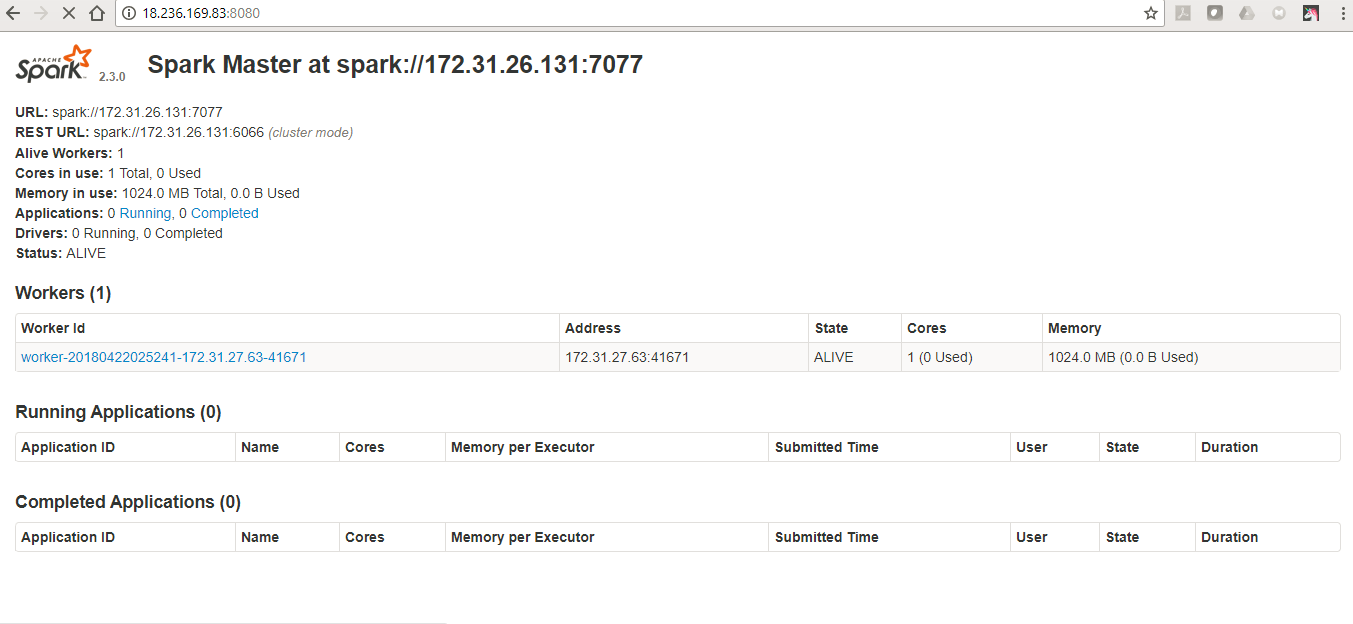
\includegraphics[width=\columnwidth]{images/sparkclusterurl.png}
\caption{EC2 instance}\label{f:spark-cluster-url}
\end{figure}

\subsection{Terminate Apache Spark Cluster}

Execute the following command on the command line to terminate Apache
Spark Cluster~\cite{hid-sp18-511-www-spark}.

\begin{verbatim}
cd ~/github/cloudmesh-community/$HID.git/project-code/
ansible-playbook site.yml --tags ``terminate``
\end{verbatim}

This command will perform following tasks:

\begin{itemize}
	\item Terminate Spark master node
	\item Terminate Spark worker node
\end{itemize}

Validate spark master and spark worker nodes have been terminated by
login to AWS~\cite{hid-sp18-511-www-aws} console.

\begin{verbatim}
\TODO{Add picture of terminated instances}
\end{verbatim}

\section{Results}

Table~\ref{t:results-table} provides the benchmark results.

\begin{table}[]
	\centering
	\caption{Results}\label{t:results-table}
	\begin{tabular}{ll} 
		\textbf{Setup} & \textbf{Duration (in minutes)} \\ 
		Apache Spark cluster deployment  & 21 mins \\
		Apache Spark cluster termination & 1 min \\
	\end{tabular}
\end{table}


\section{Conclusion}

\TODO{Put here an conclusion. Conclusion and abstracts must not have any
	citations in the section.}


\begin{acks}

  The authors would like to thank Dr.~Gregor~von~Laszewski for his
  support and suggestions to write this paper.

\end{acks}

\bibliographystyle{ACM-Reference-Format}
\bibliography{report} 

